\documentclass[ro]{problem}
\usepackage{tikz}
\title{Foc - descriere soluţie}

\input{header.tex}

\begin{document}

\maketitle

Autor: Iulia Groza

\section{Subtask 1}
\noindent Pentru primele 30 de puncte ale problemei se poate implementa o soluție brute-force. Pentru fiecare pereche de coordonate $(x, y)$ din matrice, $1 \leq x \leq N$, $1 \leq y \leq M$ se simulează independent operația de transformare a valorilor de pe linia $x$ și coloana $y$ în valori de $1$. Se determină componentele conexe din matrice, utilizând un algoritm de tip Flood fill. 

\noindent O componentă conexă este interioară matricei dacă nu conține niciun element care se află la marginea acesteia (pe prima/ultima linie/coloană).

\emph{Observație:} Componentele conexe care nu sunt interioare nu sunt de interes pentru soluție, din moment ce casele componente sunt deja salvate.

\noindent Ulterior, se verifică dacă matricea nu conține nicio componentă conexă interioară. În caz pozitiv, se afișează perechea de coordonate $(x, y)$.

\noindent Complexitatea de timp totală este $O(N^4)$.

\section{Subtask 2}
\noindent Se determină fiecare componentă conexă de case (valori de 1), utilizând analog primului subtask un algoritm de tip Flood fill. Pentru fiecare componentă în parte, determinăm liniile și coloanele minime și maxime ale elementelor componente: $(l_{min}, c_{min})$, respectiv  $(l_{max}, c_{max})$, care denotă colțul din stânga-sus, respectiv colțul din dreapta-jos ale "dreptunghiului-chenar" al componentei. Astfel, se verifică ușor dacă o componentă conține case aflate în pericol. 

\noindent În cazul componentelor de case care trebuie salvate, este necesar să determinăm din care celule putem aplica operația astfel încât să nu mai existe nicio componentă conexă interioară. Pentru un dreptunghi în matrice, posibilitățile celulelor din care acesta poate fi salvat sunt hașurate cu gri în figura de mai jos, unde dreptunghiul dat reprezintă bordarea "dreptunghiului-chenar" ($l_{min}, c_{min}$ sunt decrementate, iar $l_{max}, c_{max}$ sunt incrementate):

\begin{center}
    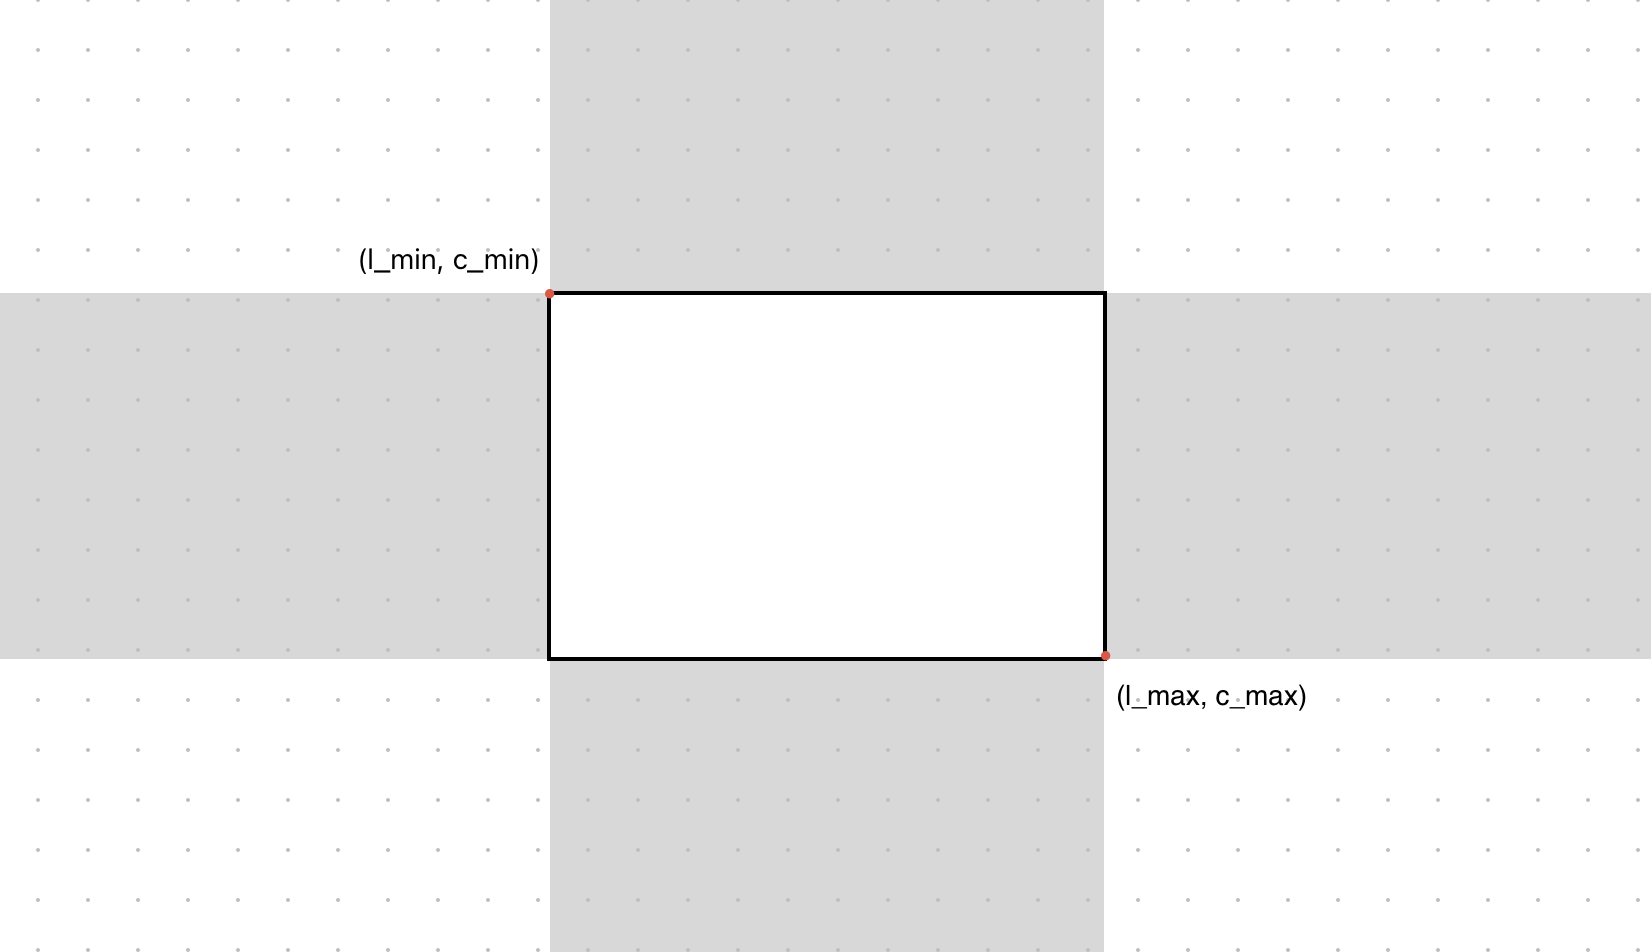
\includegraphics[width=\textwidth]{foc-descriere-coverage.png}
\end{center}

\noindent Așadar, orice celulă cu coordonatele $(x, y)$ care respectă cel puțin una din următoarele proprietăți poate salva elementele componentei din "dreptunghiul-chenar" în cauză:
\begin{itemize}
\item $l_{min} \leq x \leq l_{max}$
\item $c_{min} \leq y \leq c_{max}$
\end{itemize}

\noindent Pentru a marca în timp optim câte componente poate salva o celulă, vom folosi metoda cunoscută ca "Șmenul lui Mars" aplicat în 2D. Prin urmare, după marcarea fiecărui "dreptunghi-chenar" în celulele corespunzătoare, se utilizează sume prefix pe matrice pentru a calcula numărul total de componente care pot fi salvate dacă se aplică superputerea din celula $(x, y)$. Astfel, se poate verifica dacă o celulă poate fi soluție în timp constant.

\noindent Complexitatea de timp totală este $O(N^2)$.

\emph{Observație:} Datorită anumitor optimizări, o soluție fără update pe intervale cu complexitatea de timp $O(N^3)$ poate obține scorul maxim.

\end{document}